\documentclass[border=5pt]{standalone}
\usepackage{tikz}
\usepackage{xcolor}
\usetikzlibrary{positioning,shapes.geometric,arrows.meta,backgrounds}

\begin{document}
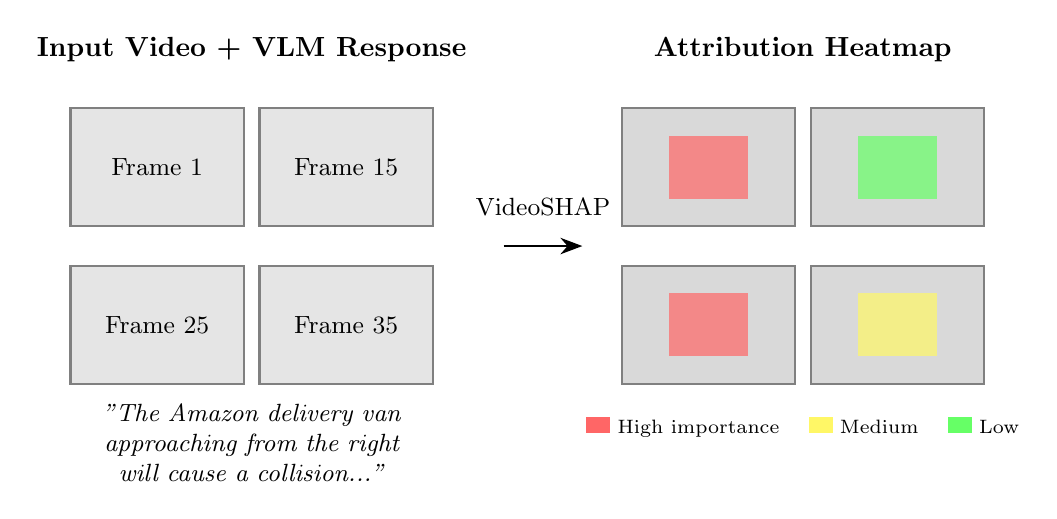
\begin{tikzpicture}[
    frame/.style={draw=gray, thick, minimum width=2.2cm, minimum height=1.5cm, fill=gray!20},
    arrow/.style={-{Stealth[scale=1.2]}, thick}
]

% Left panel - Original frames
\node[font=\bfseries] at (0, 3.5) {Input Video + VLM Response};

\node[frame] (f1) at (-1.2, 2) {};
\node[frame] (f2) at (1.2, 2) {};
\node at (f1) {\small Frame 1};
\node at (f2) {\small Frame 15};

\node[frame] (f3) at (-1.2, 0) {};
\node[frame] (f4) at (1.2, 0) {};
\node at (f3) {\small Frame 25};
\node at (f4) {\small Frame 35};

\node[text width=4.5cm, align=center, font=\small\itshape] at (0, -1.5) {
    "The Amazon delivery van approaching from the right will cause a collision..."
};

% Arrow
\draw[arrow] (3.2, 1) -- (4.2, 1);
\node[font=\small] at (3.7, 1.5) {VideoSHAP};

% Right panel - Heatmap
\node[font=\bfseries] at (7, 3.5) {Attribution Heatmap};

\node[frame, fill=gray!30] (h1) at (5.8, 2) {};
\node[frame, fill=gray!30] (h2) at (8.2, 2) {};
\node[frame, fill=gray!30] (h3) at (5.8, 0) {};
\node[frame, fill=gray!30] (h4) at (8.2, 0) {};

% Overlay colored boxes representing objects
\fill[red!60, opacity=0.7] (5.3, 1.6) rectangle (6.3, 2.4);
\fill[green!60, opacity=0.7] (7.7, 1.6) rectangle (8.7, 2.4);
\fill[red!60, opacity=0.7] (5.3, -0.4) rectangle (6.3, 0.4);
\fill[yellow!60, opacity=0.7] (7.7, -0.4) rectangle (8.7, 0.4);

% Legend
\node[font=\scriptsize] at (7, -1.3) {
    \tikz{\fill[red!60] (0,0) rectangle (0.3,0.2);} High importance \quad
    \tikz{\fill[yellow!60] (0,0) rectangle (0.3,0.2);} Medium \quad
    \tikz{\fill[green!60] (0,0) rectangle (0.3,0.2);} Low
};

\end{tikzpicture}
\end{document}
